\section{Experiments}
\label{sec:experiments}

This section evaluates whether Scene Map improves downstream manipulation policy learning beyond raw visual or geometric input. We first report main results on simulation benchmarks in sec.~\ref{sec:main_experiments}, then evaluate sim-to-real transfer in sec.~\ref{sec:real_world_experiments}. We further analyze Scene Map construction bottlenecks in sec.~\ref{sec:system_breakdown} and validate key design choices through ablations in sec.~\ref{sec:ablation_studies}.

\begin{figure}[t]
    \centering
    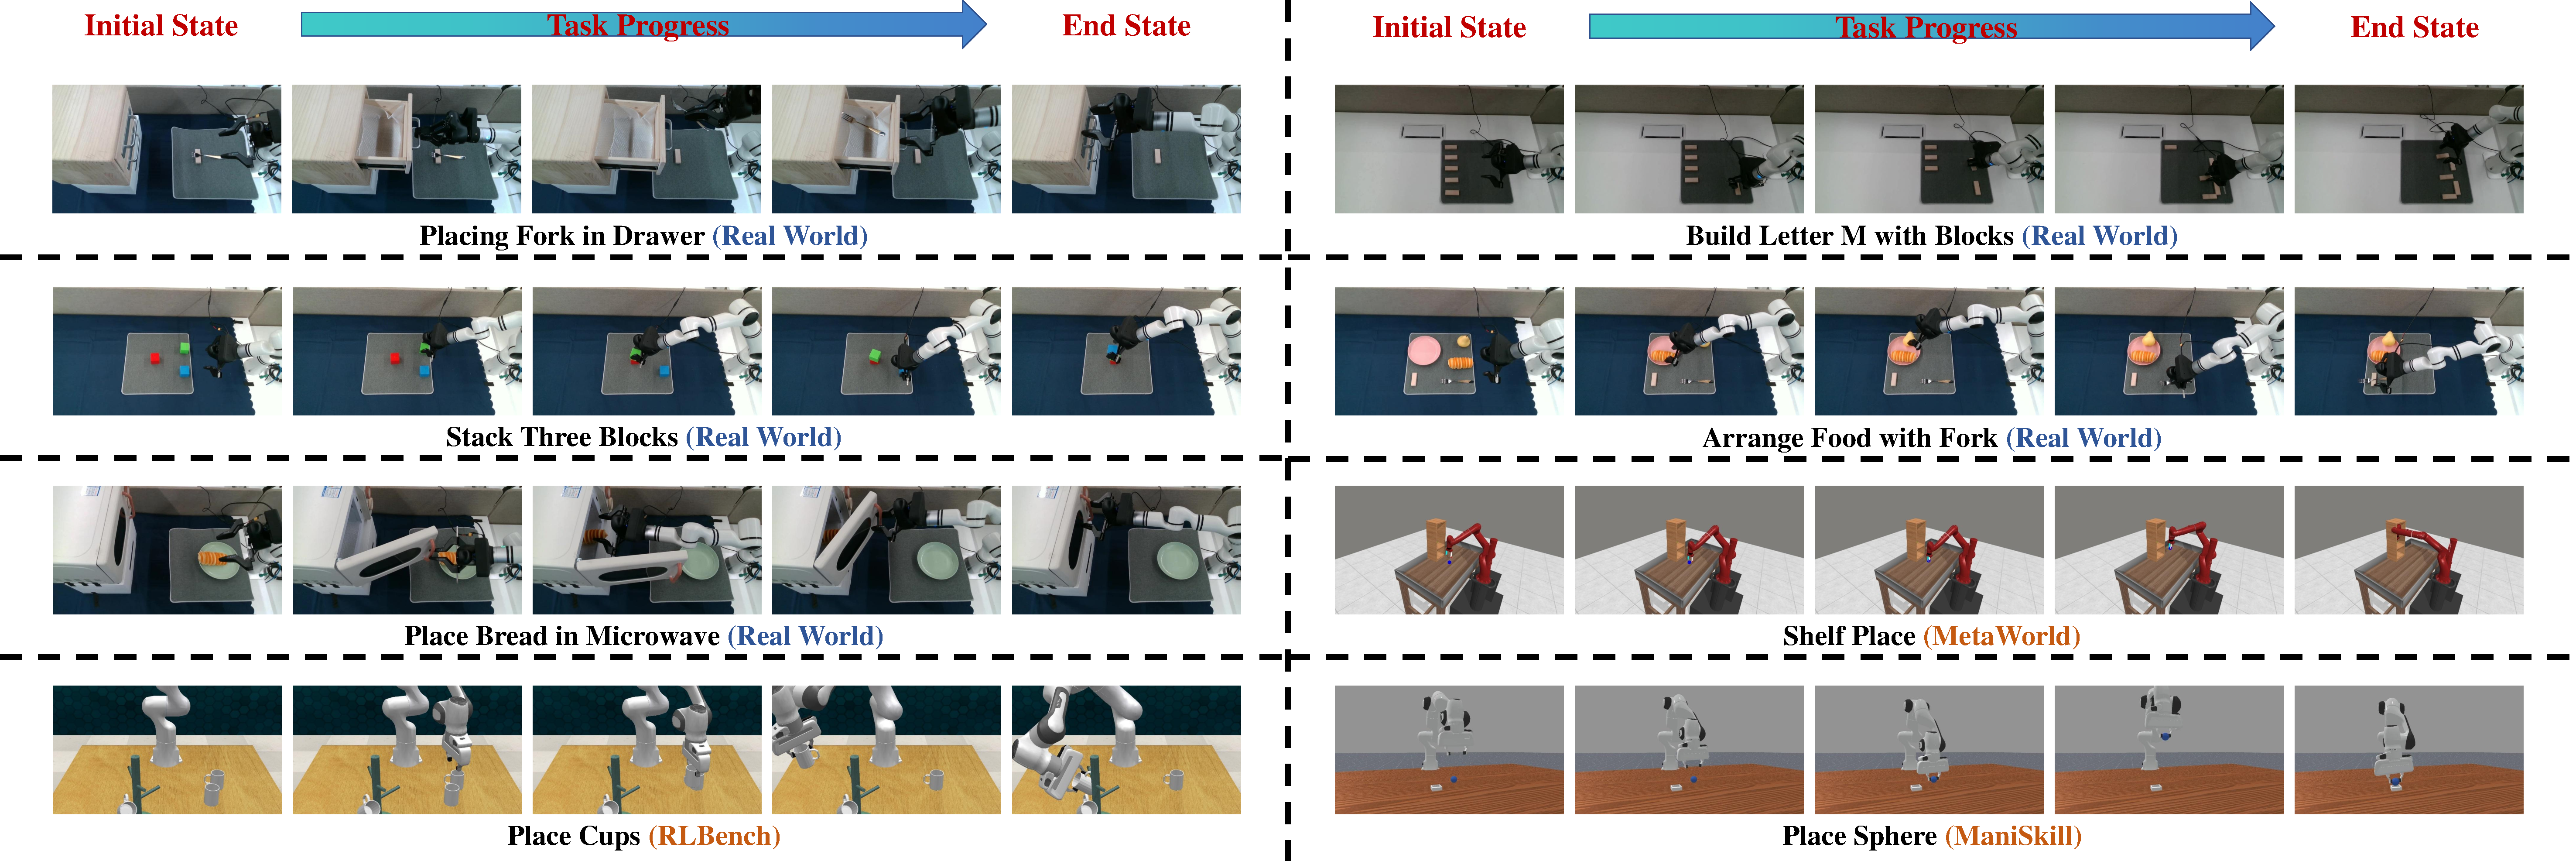
\includegraphics[width=0.95\linewidth]{figs/demonstration.pdf}
    \caption{Demonstrations of the evaluation tasks. The figure shows all five real-world tasks and representative tasks from MetaWorld~\cite{Yu2020Meta,mclean2025metaworld}, RLBench~\cite{James2020RLBench}, and ManiSkill~\cite{Gu2023ManiSkill2}, illustrating the diversity of articulated interaction, object arrangement, and geometrically constrained manipulation considered in our experiments.}
    \label{fig:demonstration}
\end{figure}

\subsection{Main Experiments in Simulation Benchmarks}
\label{sec:main_experiments}

We evaluate MapPolicy on three simulation benchmarks with complementary characteristics: MetaWorld~\cite{Yu2020Meta,mclean2025metaworld}, RLBench~\cite{James2020RLBench}, and ManiSkill~\cite{Gu2023ManiSkill2}. Together, they cover classical single-task manipulation, large-scale multi-task interaction, and tabletop manipulation.

\textbf{Experiment Settings.}
We benchmark MapPolicy on three suites.
\textbf{MetaWorld}~\cite{Yu2020Meta,mclean2025metaworld} contains 25 tasks in our evaluation and is used to test whether Scene Map helps on diverse classical MuJoCo-based manipulation problems requiring part-level interaction and precise spatial reasoning~\cite{todorov2012mujoco}.
\textbf{RLBench}~\cite{James2020RLBench} contains 18 tasks in our evaluation and is used to test whether the benefits of Scene Map persist in visually richer and more diverse multi-task settings.
\textbf{ManiSkill}~\cite{Gu2023ManiSkill2} contains six tasks from the official \textit{Table-Top 2 Finger Gripper Tasks} category, including \textit{PegInsertionSide-v1}, \textit{PlaceSphere-v1}, \textit{PlugCharger-v1}, \textit{PullCubeTool-v1}, \textit{StackCube-v1}, and \textit{StackPyramid-v1}, and is used to test MapPolicy on tabletop RGB-D manipulation with strong geometric and contact constraints.
Across all three benchmarks, the main metric is task success rate. We report mean and standard deviation across five random seeds for the main simulation results. Detailed training and evaluation protocols are provided in Appendix~\ref{app:experimental_protocols}.

\textbf{Baselines.}
We compare against strong baselines from three categories: diffusion-based policies, general-purpose visuomotor foundation policies, and 3D manipulation policies.
On MetaWorld, we compare against \textit{Diffusion Policy}~\cite{chi2024diffusionpolicy}, \textit{3D Diffusion Policy}~\cite{Ze2024DP3}, \textit{$\pi_0$}~\cite{black2026pi0visionlanguageactionflowmodel}, and \textit{Lift3D}~\cite{Jia_2025_CVPR}.
On RLBench, we compare against published baselines reported in prior work, including \textit{PerAct}~\cite{shridhar2022peract}, \textit{3D Diffuser Actor}~\cite{3d_diffuser_actor}, \textit{RVT-2}~\cite{goyal2024rvt2}, and the \textit{PDFactor} family~\cite{Tian_2025_CVPR}, using their reported numbers.
On ManiSkill, we compare against \textit{Diffusion Policy}~\cite{chi2024diffusionpolicy}, \textit{3D Diffusion Policy}~\cite{Ze2024DP3}, \textit{Octo}~\cite{octo_2023}, and \textit{$\pi_0$}~\cite{black2026pi0visionlanguageactionflowmodel}.

\begin{table*}[t]
\centering
\caption{Summary of main simulation results. We report average success rate (\%) across all evaluated tasks in each benchmark. Full per-task results are provided in Appendix~\ref{app:full_sim_results}.}
\label{tab:main_results_summary}
\small
\setlength{\tabcolsep}{6pt}
\begin{adjustbox}{max width=\textwidth}
\begin{tabular}{lc|lc|lc}
\toprule
\rowcolor{tablehead}
\multicolumn{2}{c|}{MetaWorld~\cite{Yu2020Meta,mclean2025metaworld} (25 tasks)} &
\multicolumn{2}{c|}{RLBench~\cite{James2020RLBench} (18 tasks)} &
\multicolumn{2}{c}{ManiSkill~\cite{Gu2023ManiSkill2} (6 tasks)} \\
\rowcolor{tablehead}
Method & Mean S.R. (\%) & Method & Mean S.R. (\%) & Method & Mean S.R. (\%) \\
\midrule
Diffusion Policy~\cite{chi2024diffusionpolicy} & 27.3 &
PerAct~\cite{shridhar2022peract} & 49.4 &
Diffusion Policy~\cite{chi2024diffusionpolicy} & 26.8 \\
3D Diffusion Policy~\cite{Ze2024DP3} & 51.1 &
3D Diffuser Actor~\cite{3d_diffuser_actor} & 81.4 &
3D Diffusion Policy~\cite{Ze2024DP3} & 53.8 \\
$\pi_0$~\cite{black2026pi0visionlanguageactionflowmodel} & 69.5 &
RVT-2~\cite{goyal2024rvt2} & 81.4 &
Octo~\cite{octo_2023} & 16.8 \\
\underline{Lift3D~\cite{Jia_2025_CVPR}} & \underline{78.8} &
\underline{PDFactor~\cite{Tian_2025_CVPR}} & \underline{87.3} &
\underline{$\pi_0$~\cite{black2026pi0visionlanguageactionflowmodel}} & \underline{54.0} \\
\rowcolor{tablehead}
\textbf{MapPolicy} & \textbf{93.2} &
\textbf{MapPolicy} & \textbf{94.8} &
\textbf{MapPolicy} & \textbf{73.0} \\
\bottomrule
\end{tabular}
\end{adjustbox}
\end{table*}


\begin{table}[t]
\centering
\caption{Real-world results. We report success rate (\%) over 100 trials for each real-world manipulation task. Best results are in \textbf{bold}, and second best are \underline{underlined}.}
\label{tab:real_world_results}
\small
\setlength{\tabcolsep}{4pt}
\begin{adjustbox}{max width=0.85\linewidth}
\begin{tabular}{l|c|ccccc}
\toprule
\rowcolor{tablehead}
Method & Avg. &
\shortstack{Place Fork\\in Drawer} &
\shortstack{Stack Three\\Blocks} &
\shortstack{Arrange Food\\with Fork} &
\shortstack{Place Bread\\in Microwave} &
\shortstack{Build Letter M\\with Blocks} \\
\midrule
Diffusion Policy~\cite{chi2024diffusionpolicy} & 15.4 & 12 & 6 & 41 & 18 & 0 \\
3D Diffusion Policy~\cite{Ze2024DP3} & 33.6 & 38 & 21 & 66 & 43 & 0 \\
Lift3D~\cite{Jia_2025_CVPR} & 36.2 & 41 & 25 & 69 & 46 & 0 \\
$\pi_0$~\cite{black2026pi0visionlanguageactionflowmodel} & \underline{49.8} & \underline{51} & \underline{39} & \underline{83} & \underline{61} & \underline{15} \\
\midrule
MapPolicy (Ours) & \textbf{81.4} & \textbf{87} & \textbf{78} & \textbf{95} & \textbf{84} & \textbf{63} \\
\bottomrule
\end{tabular}
\end{adjustbox}
\end{table}



\textbf{Results.}
\textbf{MetaWorld}~\cite{Yu2020Meta,mclean2025metaworld} tests classical manipulation tasks requiring actionable-part identification and local spatial reasoning. As shown in tab.~\ref{tab:main_results_summary}, MapPolicy achieves 93.2\% average success rate, outperforming the strongest prior baseline Lift3D at 78.8\%. The gains are particularly meaningful on articulated interaction, contact-rich manipulation, and precise placement. Full per-task results are provided in Appendix~\ref{app:full_sim_results}.
\textbf{RLBench}~\cite{James2020RLBench} evaluates larger-scale multi-task scenes with richer visual variation and multi-object interaction. MapPolicy reaches 94.8\% average success rate, improving over the strongest published baseline PDFactor at 87.3\%, indicating that Scene Map benefits extend beyond classical manipulation settings.
\textbf{ManiSkill}~\cite{Gu2023ManiSkill2} focuses on tabletop tasks with strong geometric constraints such as insertion, plugging, stacking, and tool use. MapPolicy obtains 73.0\% average success rate, outperforming $\pi_0$ at 54.0\% and 3D Diffusion Policy at 53.8\%, with the largest gains on tasks where explicit structure is directly relevant to action success.

\subsection{Real-World Experiments}
\label{sec:real_world_experiments}

We evaluate whether the Scene Map interface transfers from simulation to real RGB-D manipulation on a Realman 75-BF robot arm with 7 DoF and a pika gripper, running at 30 Hz. RGB-D observations are captured by an NVIDIA RealSense D415, and point clouds are constructed with Open3D~\cite{Zhou2018Open3D}. We reuse representative baselines from our simulation study for the real-world setting. In the current real-robot evaluation, we directly deploy \textit{Diffusion Policy}~\cite{chi2024diffusionpolicy} and \textit{3D Diffusion Policy}~\cite{Ze2024DP3} as the primary reproducible baselines, while \textit{$\pi_0$}~\cite{black2026pi0visionlanguageactionflowmodel} and \textit{Lift3D}~\cite{Jia_2025_CVPR} provide additional reference points for method positioning. For each real-world task, we execute each method for 100 trials and report task success rate as the main metric.


\textbf{Task Suite.}
We design five real-world tasks that cover articulated interaction, reflective-object grasping, multi-object spatial reasoning, and long-horizon arrangement.
\textit{Place Fork in Drawer} consists of four stages: opening a closed drawer, picking up a fork placed on a block, placing it into the drawer, and closing the drawer. This task is challenging because it combines articulated-object manipulation with grasping a thin, irregular, and reflective metal object.
\textit{Stack Three Blocks} requires first placing a green block on a red block and then placing a blue block on the green block. The main difficulty is maintaining the correct spatial relation across three objects during sequential stacking.
\textit{Arrange Food with Fork} consists of placing bread on a plate, placing a pear on the plate, and then placing a fork on a block stand. Although this is a more common tabletop arrangement task, it still tests compositional multi-object placement in a cluttered real scene.
\textit{Place Bread in Microwave} consists of opening the microwave door, transferring bread from a plate into the microwave, and closing the door. This task emphasizes articulated manipulation under partial occlusion and changing scene geometry.
\textit{Build Letter M with Blocks} requires arranging five blocks into a specified global shape. Unlike local pick-and-place tasks, this setting tests whether the policy can reason about a target spatial pattern and adjust placements online to satisfy the final global arrangement.

\textbf{Results.}
As shown in tab.~\ref{tab:real_world_results}, we report success rate over 100 real-robot trials for each task and each method. MapPolicy transfers robustly to the real world and is particularly effective on tasks where success depends on understanding hidden structure, articulated state, or global spatial layout. Compared with Diffusion Policy~\cite{chi2024diffusionpolicy} and 3D Diffusion Policy~\cite{Ze2024DP3}, MapPolicy produces more stable multi-step behavior on drawer and microwave tasks and better preserves the required inter-object arrangement on stacking and shape-construction tasks. These results are consistent with our central claim: explicit Scene Map helps the policy maintain a manipulation-oriented representation of object structure and spatial relations even when raw observations are noisy, partially occluded, or insufficient to reveal the full scene state.

\subsection{System Error Breakdown}
\label{sec:system_breakdown}

\begin{table}[t]
\centering
\caption{System error breakdown on MetaWorld~\cite{Yu2020Meta,mclean2025metaworld}. We use oracle replacements to identify the dominant bottleneck in MapPolicy. Oracle quantities are used only for analysis and are not part of the inference interface. $\Delta$ reports the improvement over Full MapPolicy.}
\label{tab:system_breakdown}
\small
\setlength{\tabcolsep}{6pt}
\begin{adjustbox}{max width=0.9\columnwidth}
\begin{tabular}{l|ccc|>{\columncolor{white}}c|c}
\toprule
Setting & GT Extraction & GT Object Pose & GT Structural Size & Avg. Success & $\Delta$ \\
\midrule
Full MapPolicy &  &  &  & \cellcolor{blue1}93.2 & 0.0 \\
+ GT Extraction & $\checkmark$ &  &  & \cellcolor{blue1}93.4 & +0.2 \\
+ GT Object Pose &  & $\checkmark$ &  & \cellcolor{blue2}94.0 & +0.8 \\
+ GT Structural Size &  &  & $\checkmark$ & \cellcolor{blue2}94.6 & +1.4 \\
+ GT Extraction + GT Object Pose & $\checkmark$ & $\checkmark$ &  & \cellcolor{blue1}93.4 & +0.2 \\
+ GT Extraction + GT Structural Size & $\checkmark$ &  & $\checkmark$ & \cellcolor{blue3}95.1 & +1.9 \\
+ GT Object Pose + GT Structural Size &  & $\checkmark$ & $\checkmark$ & \cellcolor{blue4}95.9 & +2.7 \\
+ GT Extraction + GT Object Pose + GT Structural Size & $\checkmark$ & $\checkmark$ & $\checkmark$ & \cellcolor{blue4}96.0 & +2.8 \\
\bottomrule
\end{tabular}
\end{adjustbox}
\end{table}


\begin{table*}[t]
\centering
% --- Left table: Scene Map contents ---
\begin{minipage}[t]{0.52\textwidth}
    \centering
    \caption{Ablation study on Scene Map representation by varying node and edge attributes on MetaWorld~\cite{Yu2020Meta,mclean2025metaworld}.}
    \label{tab:ablation_map_contents}
    \scriptsize
    \resizebox{\linewidth}{!}{
        \begin{tabular}{c|cccc|cccc|c}
        \hline
         & \multicolumn{4}{c|}{Node} & \multicolumn{4}{c|}{Edge} &  \\
        \hline
         & Geo & Pose & Sem & Aff & Type & Param & Anchor & RelPose & \textbf{Mean} \\
        \hline
        Ex1 & $\checkmark$ & - & - & - & - & - & - & - & \cellcolor{blue1}\textbf{72.4} \\
        Ex2 & $\checkmark$ & $\checkmark$ & - & - & - & - & - & - & \cellcolor{blue1}\textbf{78.1} \\
        Ex3 & $\checkmark$ & $\checkmark$ & $\checkmark$ & $\checkmark$ & - & - & - & - & \cellcolor{blue2}\textbf{83.5} \\
        Ex4 & $\checkmark$ & $\checkmark$ & $\checkmark$ & $\checkmark$ & $\checkmark$ & - & - & - & \cellcolor{blue2}\textbf{86.7} \\
        Ex5 & $\checkmark$ & $\checkmark$ & $\checkmark$ & $\checkmark$ & $\checkmark$ & $\checkmark$ & - & - & \cellcolor{blue3}\textbf{88.9} \\
        Ex6 & $\checkmark$ & $\checkmark$ & $\checkmark$ & $\checkmark$ & $\checkmark$ & $\checkmark$ & $\checkmark$ & - & \cellcolor{blue3}\textbf{91.4} \\
        \textbf{\underline{Ex7}} & $\checkmark$ & $\checkmark$ & $\checkmark$ & $\checkmark$ & $\checkmark$ & $\checkmark$ & $\checkmark$ & $\checkmark$ & \cellcolor{blue4}\textbf{93.2} \\
        \hline
        \end{tabular}
    }
\end{minipage}
\hfill
% --- Right table: encoder and fusion ---
\begin{minipage}[t]{0.46\textwidth}
    \centering
    \caption{Ablation study on map encoder and multimodal fusion design choices on MetaWorld~\cite{Yu2020Meta,mclean2025metaworld}.}
    \label{tab:ablation_encoder_fusion}
    \scriptsize
    \resizebox{\linewidth}{!}{
        \begin{tabular}{c|cccc|ccc|c}
        \hline
         & \multicolumn{4}{c|}{Map Encoder} & \multicolumn{3}{c|}{Fusion} &  \\
        \hline
         & Pool & PN & Trans. & Graph & Concat & MLP & Attn & \textbf{Mean} \\
        \hline
        Ex1 & $\checkmark$ & - & - & - & - & - & $\checkmark$ & \cellcolor{blue1}\textbf{75.6} \\
        Ex2 & - & $\checkmark$ & - & - & - & - & $\checkmark$ & \cellcolor{blue2}\textbf{82.3} \\
        Ex3 & - & - & $\checkmark$ & - & - & - & $\checkmark$ & \cellcolor{blue3}\textbf{89.1} \\
        \textbf{\underline{Ex4}} & - & - & - & $\checkmark$ & - & - & $\checkmark$ & \cellcolor{blue4}\textbf{93.2} \\
        \hline
        Ex5 & - & - & - & $\checkmark$ & $\checkmark$ & - & - & \cellcolor{blue2}\textbf{84.2} \\
        Ex6 & - & - & - & $\checkmark$ & - & $\checkmark$ & - & \cellcolor{blue3}\textbf{87.6} \\
        \textbf{\underline{Ex7}} & - & - & - & $\checkmark$ & - & - & $\checkmark$ & \cellcolor{blue4}\textbf{93.2} \\
        \hline
        \end{tabular}
    }
\end{minipage}

\par
\begin{minipage}{0.98\textwidth}
    \centering
    \scriptsize
    \textit{Note:}
    Geo = part geometry, Sem = semantic identity, Aff = affordance attributes.
    Param = continuous relation parameters, RelPose = relative pose.
    PN = PointNet~\cite{Qi2017PointNet}, Trans. = Transformer, Graph = graph encoder, Attn = attention fusion.
    Darker blue indicates better performance.
\end{minipage}
\end{table*}


MapPolicy is a multi-stage system whose final performance depends not only on downstream policy learning, but also on the quality of Scene Map construction. To identify the dominant bottleneck, we perform a system error breakdown on MetaWorld~\cite{Yu2020Meta,mclean2025metaworld} using oracle replacements. Since several error sources in MapPolicy can be independently controlled, we use a combinatorial oracle analysis instead of a single sequential replacement protocol.

\textbf{Setup.}
We analyze three independent sources of structural error: object extraction, object-pose estimation, and structural-size estimation. For each source, we replace the predicted quantity with its ground-truth counterpart and evaluate the resulting average success rate. All oracle quantities in this subsection are used only for analysis and are not part of the inference interface of MapPolicy.

\textbf{Results.}
The main result is summarized in tab.~\ref{tab:system_breakdown}, formatted as a 2D oracle matrix. The table contains three oracle columns, \textit{GT Extraction}, \textit{GT Object Pose}, and \textit{GT Structural Size}, together with one performance column, \textit{Avg. Success}. The rows enumerate all combinations of the three oracle sources.
This analysis should be read in two stages. First, the single-factor replacements reveal which structural error source is the dominant independent bottleneck. Second, the joint replacements reveal whether different error sources interact strongly or contribute largely independent errors. This subsection therefore identifies which part of the MapPolicy pipeline deserves the highest priority for improvement.


\subsection{Ablation Studies}
\label{sec:ablation_studies}



\begin{table*}[t]
\centering
\caption{Ablation study on training losses on MetaWorld~\cite{Yu2020Meta,mclean2025metaworld}. Map Attr. GT supervises the scene-dependent node and edge attributes used to instantiate Scene Map, Chamfer supervises map-induced point-cloud geometry, and Physical enforces relation-specific constraints.}
\label{tab:ablation_loss_presence}
\scriptsize
\setlength{\tabcolsep}{4pt}
\begin{adjustbox}{max width=\textwidth}
\begin{tabular}{c|cccc|c@{\hspace{12pt}}c|cccc|c}
\toprule
 & \multicolumn{4}{c|}{Loss Terms} &  &  & \multicolumn{4}{c|}{Loss Terms} &  \\
\cmidrule(lr){2-5} \cmidrule(lr){8-11}
Setting & Action & Map Attr. GT & Chamfer & Physical & Avg. Success &
Setting & Action & Map Attr. GT & Chamfer & Physical & Avg. Success \\
\midrule
Ex1 & $\checkmark$ & - & - & - & \cellcolor{blue1}80.6 &
Ex5 & $\checkmark$ & $\checkmark$ & $\checkmark$ & - & \cellcolor{blue2}88.7 \\
Ex2 & $\checkmark$ & $\checkmark$ & - & - & \cellcolor{blue1}83.4 &
Ex6 & $\checkmark$ & $\checkmark$ & - & $\checkmark$ & \cellcolor{blue3}89.5 \\
Ex3 & $\checkmark$ & - & $\checkmark$ & - & \cellcolor{blue2}84.1 &
Ex7 & $\checkmark$ & - & $\checkmark$ & $\checkmark$ & \cellcolor{blue4}\underline{92.4} \\
Ex4 & $\checkmark$ & - & - & $\checkmark$ & \cellcolor{blue1}82.8 &
\textbf{\underline{Ex8}} & $\checkmark$ & $\checkmark$ & $\checkmark$ & $\checkmark$ & \cellcolor{blue4}\textbf{93.2} \\
\bottomrule
\end{tabular}
\end{adjustbox}
\end{table*}


We design ablations to answer three questions: whether explicit Scene Map is necessary as a representation, how Scene Map should be encoded and fused with visual information, and which supervision terms make the learned map most useful for downstream control.

\textbf{Scene Map Representation.}
We first evaluate which contents inside Scene Map are most important for policy learning. We conduct this ablation on MetaWorld~\cite{Yu2020Meta,mclean2025metaworld} and keep the policy backbone and training recipe fixed, changing only the attributes included in the map representation. Table~\ref{tab:ablation_map_contents} progressively adds node attributes, including part geometry, pose, semantic identity, and affordance-related information, and then edge attributes, including relation type, continuous relation parameters, anchor references, and relative pose. This comparison separates the contribution of part-level node descriptors from the contribution of explicit cross-part relations. If edge attributes provide additional gains beyond node-only representations, the conclusion is that Scene Map helps not only by describing object parts, but also by modeling the structural and physical relations among them.



\textbf{Structure-Aware Encoder and Fusion.}
Given a Scene Map, the next question is how it should be encoded and fused with visual information. We therefore study both the choice of map encoder and the choice of fusion strategy. Table~\ref{tab:ablation_encoder_fusion} compares four encoders while keeping the Scene Map representation fixed: \textit{Pooling}, \textit{PointNet}~\cite{Qi2017PointNet}, \textit{Transformer}~\cite{Kim2021Transformer}, and \textit{Graph Encoder}. This comparison tests whether relation-aware graph encoding is necessary to fully exploit the node-edge structure of Scene Map. We then fix the best map encoder and compare three fusion strategies: \textit{Concat}, \textit{MLP fusion}, and \textit{Attention fusion}. These results show whether the information in Scene Map can be effectively used by naive concatenation or whether a stronger fusion mechanism is needed to integrate structural and visual cues for downstream action prediction.

\textbf{Loss Design.}
We keep action imitation enabled and ablate three auxiliary losses: map-attribute supervision, point-cloud Chamfer supervision, and physical constraint regularization. Table~\ref{tab:ablation_loss_presence} shows that each auxiliary loss improves over action imitation alone, while combining Chamfer supervision with physical constraints gives the strongest partial combination and using all three losses achieves the best performance.

